\chapter{Fundamentação Teórica}


\section{Sistemas de Controle}

Os sistemas de controle constituem um conjunto integrado de componentes que visam a regulação e a supervisão do
comportamento de sistemas dinâmicos.
Essenciais em uma muitas de aplicações práticas, são empregados para assegurar a estabilidade operacional e a precisão
de resposta a perturbações.
A operação desses sistemas pode ser realizada sob duas configurações principais: sistemas de malha aberta,
onde não há realimentação do estado do sistema, e sistemas de malha fechada, que se caracterizam pela incorporação de
realimentação na estratégia de controle.
A eficiência de um sistema de controle é determinada pela sua habilidade em alcançar e sustentar um estado operacional
desejado, reduzindo desvios e oscilações indesejadas.
A precisão com que um sistema de controle atinge e mantém a saída desejada, apesar das flutuações nos parâmetros ou nas
condições ambientais, é um indicador crítico de seu desempenho. \cite{ogata2010engenharia}.

Um sistema de controle em malha aberta opera sem a leitura de qualquer variável.
Nesse arranjo, o controlador atua baseado apenas no sinal de entrada, sem ajustar sua ação em resposta a distúrbios ou
variações na saída.
Um exemplo clássico é o controle de velocidade de um motor, onde a quantidade de combustível é ajustada apenas com base
na velocidade desejada, sem considerar a velocidade real do motor. \cite[Cap 2.3]{ogata2010engenharia}.

Em contraste, um sistema de controle em malha fechada inclui um ciclo de realimentação, onde a saída é continuamente
monitorada e comparada com o sinal de referência.
A diferença entre esses dois, conhecida como erro, é utilizada pelo controlador para ajustar o sinal de controle e,
assim, minimizar o erro. \cite[Cap 2.3]{ogata2010engenharia}.

\begin{figure}[H]
    \centering
    \caption{Diagrama de blocos de um sistema de malha fechada}
    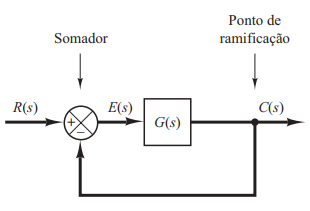
\includegraphics[scale=1]{figuras/closed_loop}
    \label{fig:closed_loop}
    \\
    \vspace{0cm}\hspace{0cm}\small{Fonte: \cite[Fig 2.3]{ogata2010engenharia}}
\end{figure}

Onde:
\begin{itemize}
    \item $R(s)$: Representa o sinal de referência.
    \item $G(s)$: Representa o sistema sistema.
    \item $C(s)$: Representa a saida.
    \item $E(s)$: É o erro ou a diferença entre $R(s)$ e $C(s)$.
\end{itemize}

\subsection{Modelo}

De acordo com \cite{CoelhoIdentificacao}, em controle de processos, um modelo não busca ser uma réplica exata do
sistema real, mas sim uma representação adequada para uma aplicação específica.
A modelagem é um procedimento que visa obter um conjunto de equações matemáticas que descrevem a dinâmica do sistema,
permitindo responder a questões sobre o sistema sem a realização de experimentações físicas.
A simplicidade é muitas vezes uma virtude na modelagem de processos, pois modelos excessivamente complexos podem
não ser necessários para capturar a dinâmica essencial do sistema para fins de controle.

A função de transferência é uma forma comum de representar o modelo de um sistema em controle de processos.
Ela é definida como a razão entre a transformada de Laplace da saída e da entrada do sistema,
sendo uma razão de dois polinômios em $s$, onde $s$ é a variável complexa da transformada de Laplace.
Esta representação é particularmente útil para a análise e o projeto de sistemas de controle,
pois permite uma avaliação clara da resposta do sistema a diferentes tipos de sinais de entrada,
como impulso, degrau, rampa e senoidal.

Um modelo clássico e comumente utilizado para representação de sistemas de controle de primeira ordem com atraso é
representado pela seguinte função de transferência:
\begin{equation}
    \label{eq:firstordertf}
    G(s) = \frac{K}{\tau s + 1}e^{-\theta s}
\end{equation}
onde cada termo tem um significado específico:
\begin{itemize}
    \item $G(s)$: Função de transferência do sistema no domínio da frequência.
    \item $K$: Ganho do sistema, que determina a amplitude da saída em relação à entrada.
    \item $\tau$: Constante de tempo do sistema, que indica a rapidez com que o sistema responde a uma entrada.
    \item $\theta$: Tempo de atraso, que representa o tempo que leva para a resposta do sistema começar após uma entrada.
    \item $s$: Variável complexa da Transformada de Laplace, usada para transformar funções do tempo para o domínio da frequência.
\end{itemize}

Este modelo é particularmente útil para descrever sistemas onde há um atraso perceptível entre a ação de controle e a
resposta observada.
A exponencial negativa \( e^{-\theta s} \) incorpora o atraso no modelo, deslocando a resposta do sistema no tempo.
A constante de tempo \( \tau \) e o ganho \( K \) são parâmetros fundamentais que influenciam a dinâmica do sistema.
Através de simulações baseadas neste modelo, é possível prever o comportamento do sistema sob diferentes
condições operacionais e ajustar o projeto de um controlador antes da implementação real.

No contexto da automação industrial, os modelos matemáticos são empregados para previsão, análise e projeto de sistemas
de controle, essenciais para a sintonia de controladores e a otimização de processos.

\subsection{Controlador}

Dentro do universo dos sistemas de controle, um controlador é um componente crucial que modula a entrada de um sistema
para alcançar a saída desejada.
Ele atua ajustando o sinal de controle em resposta às variações da saída, visando minimizar a diferença entre a saída
observada e a saída desejada, conhecida como sinal de referência.
Os controladores podem ser classificados de acordo com suas ações de controle, alguns exemplos são controladores,
como on-off, proporcionais, integrais, proporcional-integrais (PI), proporcional-derivativos (PD) e
proporcional-integral-derivativos (PID), cada um com características distintas que os tornam adequados para diferentes
aplicações industriais. \cite[Cap 2.3]{ogata2010engenharia}.

%chck
O controlador PID é um dos tipos mais prevalentes de controladores em sistemas de controle, caracterizado pela sua
função de transferência,
\begin{equation}
    \label{eq:ctrlr}
    G_c(s) = K_p + \frac{K_i}{s} + K_d s
\end{equation}
onde \( K_p \), \( K_i \), e \( K_d \) representam os ganhos proporcional, integral e derivativo, respectivamente.
O termo proporcional \( K_p \) determina a reação do controlador à magnitude atual do erro,
o termo integral \( K_i \) acumula o erro ao longo do tempo, visando eliminar o erro estático,
e o termo derivativo \( K_d \) responde à taxa de variação do erro, antecipando o comportamento futuro.
A escolha adequada desses parâmetros é crucial: um \( K_p \) elevado pode acelerar a resposta do sistema, mas
potencialmente à custa da estabilidade;
um \( K_i \) excessivo pode introduzir oscilações devido ao atraso na resposta;
e um \( K_d \) significativo pode melhorar a estabilidade e a resposta rápida, mas é sensível ao ruído do sinal de
medição.
O ajuste dos três efeitos do controlador PID é essencial para otimizar o desempenho do sistema, tanto em resposta
transitória quanto em regime estacionário. \cite[Cap 2.3 e 8]{ogata2010engenharia}.

Vale ressaltar que controladores como P, PI e PD, podem ser vistos como um controlador PID onde o ganho para os
parâmetros não citados é ajustado para zero.

\subsection{Métodos de Identificação}

Segundo \cite[Cap 2]{CoelhoIdentificacao}, métodos de identificação de sistemas referem-se ao conjunto de técnicas
utilizadas para construir modelos matemáticos que capturam a dinâmica de sistemas reais a partir de dados de entrada e
saída.
Estes métodos buscam determinar os parâmetros do sistema que melhor se ajustam às medidas observadas,
permitindo que o modelo matemático reproduza o comportamento do sistema.
A identificação pode ser conduzida de duas formas principais: \textit{off-line} e \textit{on-line}.

Na identificação \textit{off-line}, coleta-se um conjunto de dados de entrada e saída, comumente referidos como dados discretos,
processados posteriormente para estimar os parâmetros do modelo.
Este processo não possui restrições de tempo computacional e é tipicamente realizado utilizando algoritmos
não-recursivos.
Já a identificação \textit{on-line} ajusta os parâmetros do modelo em tempo real, sem a necessidade de armazenar previamente as
medidas.
Utiliza-se um algoritmo recursivo que atualiza os parâmetros após cada amostra coletada,
o que é particularmente útil para sistemas que mudam com o tempo ou quando é necessário um ajuste contínuo do modelo.

Devido ao escopo deste trabalho, métodos de identificação \textit{on-line} não serão abordados, apenas métodos \textit{off-line} baseados
nos dados discretos de resposta do sistema.

\subsubsection{Ziegler Nichols}\label{subsubsec:znfun}

O método Ziegler-Nichols é um clássico da literatura para identificação de modelos dinâmicos de
processos industriais.
Desenvolvido por Ziegler e Nichols em 1942 \cite[Cap 4]{CoelhoIdentificacao}.

O processo de identificação de um modelo por esse método envolve a análise da resposta de um sistema a um sinal
degrau, para obter os parâmetros da equação\eqref{eq:firstordertf}, $K$, $\tau$ e $\theta$ e criar
a função de transferência representativa do modelo do sistema analisado.

Os parâmetros são calculados conforme indicado pela figura a seguir:
\begin{figure}[H]
    \centering
    \caption{Métodos de ZN e HAG para a modelagem de processos de primeira ordem}
    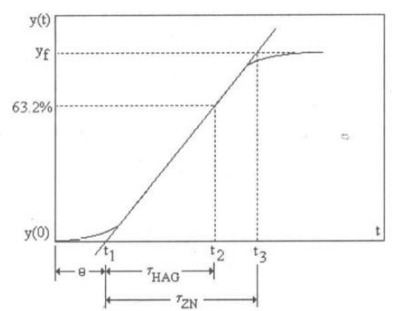
\includegraphics[scale=0.3]{figuras/zn_hg_ident_meth}
    \label{fig:zn_hg_ident_meth}
    \\
    \vspace{0cm}\hspace{0cm}\small{Fonte: \cite[Fig 4.3]{CoelhoIdentificacao}}
\end{figure}

A reta traçada corresponde à tangente no ponto de máxima inclinação da curva de reação.

A constante de tempo $\tau$ é determinada pelo intervalo de tempo entre $t_1$, e o instante
$t_3$, onde a reta tangente toca o eixo $t$, e onde cruza com a reta $y(t) = y_f$,
respectivamente.
O valor de  $\theta$ é considerado como $t_1$, o intervalo entre a aplicação do sinal degrau e o
momento em que a reta tangente toca o eixo $t$.
Por fim o valor de $K$ pode ser obtido a través da equação,
\begin{equation}
    \label{eq:dydu}
    K = \frac{\Delta y}{\Delta u}
\end{equation}
Ou seja $y_f$ dividido pelo valor do sinal degrau. \cite[Cap 4]{CoelhoIdentificacao}.

\subsubsection{Hagglund}

O método Hagglund é mais um clássico da literatura para identificação de modelos dinâmicos de
processos industriais.
Desenvolvido por Hagglund em 1991 \cite[Cap 4]{CoelhoIdentificacao}.

A identificação de modelo pelo método de Hägglund é muito similar a de Ziegler e Nichols (\ref{subsubsec:znfun}), com a
única diferença sendo que $\tau$ é determinado pelo intervalo de tempo entre $t_1$, e o instante $t_2$, sendo $t_2$
o momento em que a curva de resposta alcança o valor $y(t) = y(0) + 0.632y_f$, ou seja $63.2\%$ do valor de regime.
Isso pode ser visualizado na figura \ref{fig:zn_hg_ident_meth}.

\subsubsection{Smith}\label{subsubsec:smfun}

Desenvolvido por Smith em 1985, o método Smith, assim como os métodos Hagglund e Ziegler-Nichols, busca encontrar
valores para os parâmetros $K$, $\tau$ e $\theta$ e criar a função de transferência representativa do modelo do sistema
analisado \cite[Cap 4]{CoelhoIdentificacao}.

\begin{figure}[H]
    \centering
    \caption{Método de Smith para a modelagem de processos de primeira ordem}
    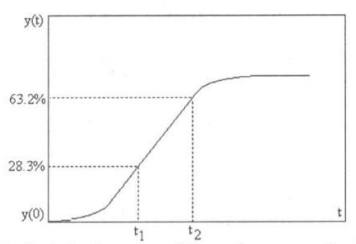
\includegraphics[scale=0.3]{figuras/sm_ident_meth}
    \label{fig:sm_ident_meth}
    \\
    \vspace{0cm}\hspace{0cm}\small{Fonte: \cite[Fig 4.3]{CoelhoIdentificacao}}
\end{figure}

Na figura \ref{fig:sm_ident_meth} podem ser observados os momentos $t1$ e $t2$, eles correspondem a passagem da resposta
pelos pontos $y(t) = y(0) + 0.283y(\infty)$ e $y(t) = y(0) + 0.632y(\infty)$, respectivamente.

As constantes podem então ser utilizadas para o cálculo da constante de tempo $\tau$ e do valor de $\theta$,
conforme as seguintes equações:
\begin{equation}
    \label{eq:smtau}
    \tau = 1.5*(t_2 - t_1)
\end{equation}
\begin{equation}
    \label{eq:smtheta}
    \theta = t_2 - \tau
\end{equation}

Por fim o valor de $K$ pode ser obtido através da equação \eqref{eq:dydu}.

\subsubsection{Sundaresan Krishnaswamy}

O método de Sundaresan e Krishnaswamy, desenvolvido em 1977 é bastante similar ao método Smith \ref{subsubsec:smfun}.
Apresentando algumas alterações nos valores para o cácluculo das constantes de tempo $t1$ e $t2$, calculadas como
$y(t) = y(0) + 0.353y(\infty)$ e $y(t) = y(0) + 0.853y(\infty)$, respectivamente, como pode ser visto na figura
\ref{fig:sd_kr_ident_meth} \cite[Cap 4]{CoelhoIdentificacao}:


\begin{figure}[H]
    \centering
    \caption{Método de Sundaresan e Krishnaswamy para a modelagem de processos de primeira ordem }
    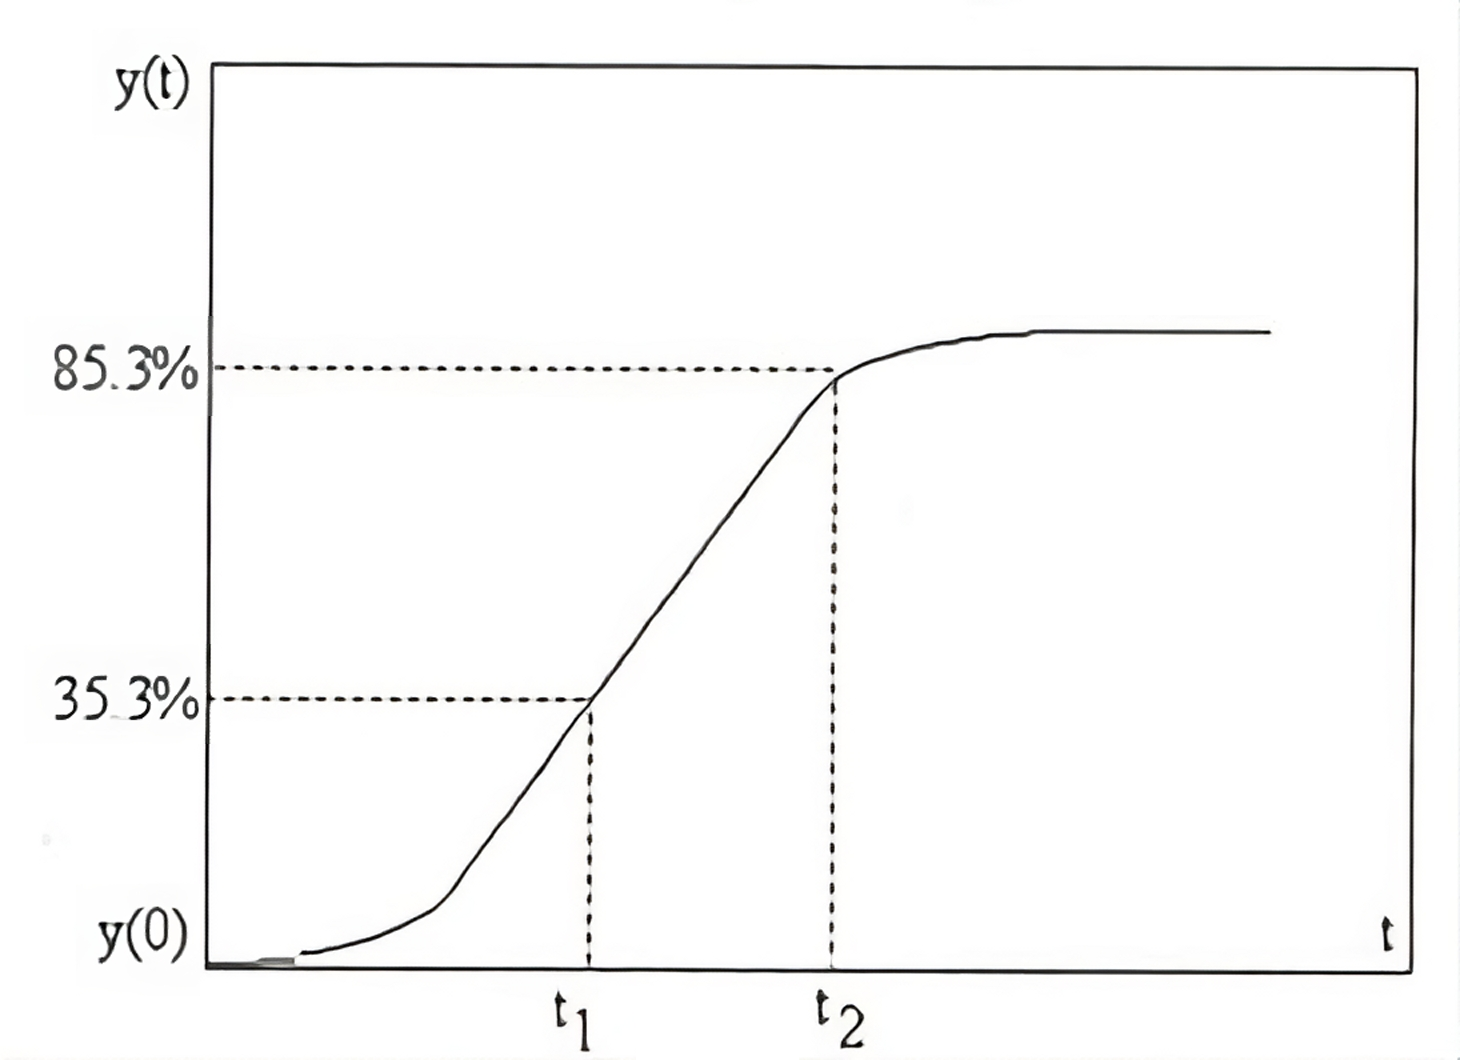
\includegraphics[scale=0.3]{figuras/sd_kr_ident_meth}
    \label{fig:sd_kr_ident_meth}
    \\
    \vspace{0cm}\hspace{0cm}\small{Fonte: \cite[Fig 4.3]{CoelhoIdentificacao}}
\end{figure}

Além de ter diferenças nas equações de $\tau$ e $\theta$, como pode ser visto nas equações \eqref{eq:sktau} e
\eqref{eq:sktheta}:
\begin{equation}
    \label{eq:sktau}
    \tau = 0.67*(t_2 - t_1)
\end{equation}
\begin{equation}
    \label{eq:sktheta}
    \theta = 1.3t_1 - 0.29t_2
\end{equation}

\subsubsection{Nishikawa}

Um último um método clássico da literatura para Identificação de modelos é o desenvolvido por Nishikawa em 1984.
A pesar de buscar os mesmos parâmetros que os métodos anteriores, estes parâmetros são obtidos através de áreas
delimitadas pela curva de resposta a sinal degrau, pelo valor de regime e pela constante de tempo $t_0$, como pode ser
observado na figura \ref{fig:ni_ident_meth}.


\begin{figure}[H]
    \centering
    \caption{Método de Nishikawa para a modelagem de processos de primeira ordem}
    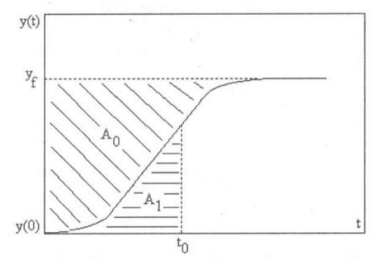
\includegraphics[scale=0.3]{figuras/ni_ident_meth}
    \label{fig:ni_ident_meth}
    \\
    \vspace{0cm}\hspace{0cm}\small{Fonte: \cite[Fig 4.3]{CoelhoIdentificacao}}
\end{figure}

As áreas e a constante de tempo podem ser calculadas conforme as seguintes equações:

\begin{equation}
    \label{eq:nia0}
    A_0 = \int_{0}^{\infty} { \Delta y(\infty) - \Delta y(t) } dt
\end{equation}
\begin{equation}
    \label{eq:nia1nt0}
    A_1 = \int_{0}^{t_0} \Delta y(t) dt \;\; ; \;\; t_0 = \frac{A_0}{\Delta y(\infty)}
\end{equation}

Com isto, podem ser obtodas as constantes $\tau$ e $\theta$:
\begin{equation}
    \label{eq:nitau}
    \tau = \frac{A_1}{0.368\Delta y(\infty)}
\end{equation}
\begin{equation}
    \label{eq:nitheta}
    \theta = t_0 - \tau
\end{equation}

Da mesma forma que os outros métodos, $K$ pode ser obtido através da equação \eqref{eq:dydu}.

\subsection{Métodos de Aproximação de Controlador PID}

A sintonia de controladores PID é um componente crucial no desenvolvimento de sistemas de controle automatizados,
fundamental para assegurar a eficiência e a estabilidade operacional.
A importância da sintonia reside na sua capacidade de ajustar o comportamento do sistema de controle para atender às
especificações de desempenho, como precisão, rapidez de resposta e estabilidade a longo prazo.
A sintonia adequada consegue compensar as incertezas inerentes ao modelo do sistema e as variações ambientais,
garantindo que o sistema mantenha seu desempenho ótimo sob uma gama de condições operacionais.
\cite{apostpidsint}.

Realizar a sintonia de um controlador PID envolve a aproximação dos ganhos do controlador capazes de causar o efeito no
sistema.
Para isso é comumente feita a análise o modelo do sistema a ser controlado.
Através da análise do modelo, é possível prever como o sistema responde a diferentes configurações de controle e
identificar os parâmetros de ganho que resultarão na resposta desejada.
Este processo de aproximação dos ganhos, permite a sintonia do sistema, assegurando que o controlador PID opere de forma
eficiente, mantendo a saída do sistema nos parâmetros desejados, minimizando o erro e otimizando a resposta a
perturbações. \cite{apostpidsint}.

\subsubsection{Ziegler Nichols}\label{subsubsec:znctr}

Proposto por Ziegler e Nichols, como uma forma de obter os ganhos de controlador para os modelos itentificados
pelo seu método de indentificação (\ref{subsubsec:znfun}), o objetivo deste método é obter parâmetros de ganho PID que
façam a sintonia do controlador \cite{apostpidsint}.

Em espessífico, este método se baseia na curva de reação do sistema a resposta de sinal degrau, que é
exatamente o que o resultado da identificação por Ziegler Nichols obtém, utilizando os parâmetros $K$, $\tau$ e $\theta$
para análise.

Desta forma, são aplicadas as fórmulas do método de acordo com a tabela \ref{tab:zncntb}.

\begin{table}[h]
    \begin{center}
        \begin{tabular}{ | l | c | c | c | }
            \hline
            {\textbf{Controlador}} & {$K_P$}                               & {$T_I$}                & {$T_D$}       \\
            \hline
            {\textbf{P}}           & {$\frac{1}{K}\frac{\tau}{\theta}$}    & {$\infty$}             & {$0$}         \\
            \hline
            {\textbf{PI}}          & {$0.9\frac{1}{K}\frac{\tau}{\theta}$} & {$\frac{\theta}{0.3}$} & {$0$}         \\
            \hline
            {\textbf{PID}}         & {$1.2\frac{1}{K}\frac{\tau}{\theta}$} & {$2\theta$}            & {$0.5\theta$} \\
            \hline
        \end{tabular}
        \caption{Método de Ziegler e Nichols para Curva de Reação}
        \label{tab:zncntb}
    \end{center}
\end{table}

Os valores de $T_I$ e $T_D$ são $1/K_i$ e $1/K_d$, respectivamente.

\subsubsection{Cohen Coon}

Criado por Cohen e Coon como uma forma de obter os ganhos de controlador, de forma similar ao método de Ziegler e Nichols
(\ref{subsubsec:znctr}), para modelos clássicos de primeira ordem com atraso.
Utiliza a seguinte tabela para determinar os ganhos de controlador PID:

\begin{table}[h]
    \begin{center}
        \begin{tabular}{ | l | c | c | c | }
            \hline
            {\textbf{Controlador}} & {$K_P$}                               & {$T_I$}                & {$T_D$}       \\
            \hline
            {\textbf{P}}           & {$\frac{1}{K}\frac{\tau}{\theta}[1+\frac{\theta}{3\tau}]$}    & {$\infty$}             & {$0$}         \\
            \hline
            {\textbf{PI}}          & {$\frac{1}{K}\frac{\tau}{\theta}[0.9+\frac{\theta}{12\tau}]$} & {$\frac{\theta [30+3 \frac{\theta}{\tau}]}{9+20 \frac{\theta}{\tau}}$} & {$0$}         \\
            \hline
            {\textbf{PID}}         & {$\frac{1}{K}\frac{\tau}{\theta}[\frac{16\tau+3\theta}{12\tau}]$} & {$\frac{\theta [32+6 \frac{\theta}{\tau}]}{13+8 \frac{\theta}{\tau}}$}            & {$\frac{4 \theta}{11+2 \frac{\theta}{\tau}}$} \\
            \hline
        \end{tabular}
        \caption{Método de Cohen e Coon para Curva de Reação}
        \label{tab:cccntb}
    \end{center}
\end{table}

Os valores de $T_I$ e $T_D$ são $1/K_i$ e $1/K_d$, respectivamente.

\section{Implementação em Python}

Introdução sobre técnicas e ferramentas para implementação de uma lib em python

\subsection{Bibliotecas em Python}

Fundamentação Bibliotecas em Python (cite pip and pypi)

\subsection{Documentação de código}

Fundamentação Documentação de código (sphinx, rtd)

\subsection{Controle em Python}

Fundamentação Controle em Python (control)

\subsection{Outras Bibliotecas}

Fundamentação Outras libs usadas

\subsection{Ferramentas Auxiliares ao Desenvolvimento}


